\documentclass[onecolumn, draftclsnofoot,10pt, compsoc]{IEEEtran}
\hbadness=1000 % suppress warnings
\usepackage{graphicx}
\usepackage{url}
\usepackage{setspace}
\usepackage{hyperref}
\usepackage{listings}
\usepackage{geometry}
\usepackage{longtable}
\usepackage{float}


\geometry{textheight=9.5in, textwidth=7in}

% 1. Fill in these details
\def \CapstoneTeamName{			}
\def \CapstoneTeamNumber{		69}
\def \GroupMemberOne{			Kin-Ho Lam}
\def \CapstoneProjectName{		Depth Sensing with Computer Vision and Lidar}
\def \CapstoneSponsorCompany{	Oregon State University}
\def \CapstoneSponsorPerson{	D. Kevin McGrath}


% 2. Uncomment the appropriate line below so that the document type works
\def \DocType{
	Spring Midterm Progress Report
}

\newcommand{\NameSigPair}[1]{\par
	\makebox[2.75in][r]{#1} \hfil 	\makebox[3.25in]{\makebox[2.25in]{\hrulefill} \hfill		\makebox[.75in]{\hrulefill}}
	\par\vspace{-12pt} \textit{\tiny\noindent
		\makebox[2.75in]{} \hfil		\makebox[3.25in]{\makebox[2.25in][r]{Signature} \hfill	\makebox[.75in][r]{Date}}}}
% 3. If the document is not to be signed, uncomment the RENEWcommand below
\renewcommand{\NameSigPair}[1]{#1}
\newcommand\captionof[1]{\def\@captype{#1}\caption}
%%%%%%%%%%%%%%%%%%%%%%%%%%%%%%%%%%%%%%%
\graphicspath{{images/}}
\begin{document}
	\begin{titlepage}
		\pagenumbering{gobble}
		\begin{singlespace}
			\centering
			
\includegraphics[height=4cm,natwidth=345,natheight=435]{images/osu_logo.png}
			\hfill 
			% 4. If you have a logo, use this includegraphics command to put it on the coversheet.
			%\includegraphics[height=4cm]{CompanyLogo}   
			\par\vspace{.2in}
			\centering
			\scshape{
				\huge Senior Design Capstone \DocType \par
				{\large\today}\par
				\vspace{.5in}
				\textbf{\Huge\CapstoneProjectName}\par
				\vfill
				{\large Prepared for}\par
				\Huge \CapstoneSponsorCompany\par
				\vspace{5pt}
				{\Large\NameSigPair{\CapstoneSponsorPerson}\par}
				{\large Prepared by }\par
				Group\CapstoneTeamNumber\par
				% 5. comment out the line below this one if you do not wish to name your team
				\CapstoneTeamName\par 
				\vspace{5pt}
				{\large
					\NameSigPair{\GroupMemberOne}\par
				}
				\vspace{20pt}
			}
			\begin{abstract}  
 				Depth Sensing with Computer Vision and Lidar proposes combining computer vision and lidar to create a reliable depth sensor.
				This document details its project member's progress toward a final design.
			\end{abstract}     
		\end{singlespace}
	\end{titlepage}
\section{Table of Contents}
\tableofcontents
\bibliographystyle{IEEEtran}
\bibliography{ref}
\clearpage

\begin{singlespace}
	\section{Definitions}
		\subsection{IR}\label{def:IR}
		IR refers to the infrared light spectrum.

		\subsection{IR Depth Sensor}\label{def:depthsensor}
		A device that calculates distances by emitting infrared patterns. 
		
		\subsection{lidar}\label{def:lidar}
		Light Detection And Ranging - A method that uses lasers to measure distance
		
		\subsection{Microsoft Kinect}\label{def:kinect}
		A product that uses an IR Depth sensor to measure distances.
		Referred as a benchmark.
		
		\subsection{Logitech Brio Webcam}\label{def:brio}
		Webcam made by Logitech. \cite{logitech}
		
		\subsection{RPLidar A1}\label{def:rplidar}
		A budget lidar device made by Slamtec. \cite{slamtec}

		\subsection{Leddar M16}\label{def:m16}
		A solid-state lidar device made by Leddar. \cite{Leddartech}

		\subsection{Computer Vision }\label{def:vision}
		The methods for acquiring, processing, analyzing, and classifying digital images and extracting information.

		
	\section{Project Purpose}
		Infrared (IR) depth sensors such as the model used in Microsoft's Kinect \ref{def:kinect} can quickly calculate distances in indoor scenarios.
		However, IR depth sensors can be confused by other infrared emitting sources such as other IR depth sensors or natural sunlight.
		For these reasons, IR depth sensors cannot be used in self-driving cars, outdoor robots, or any any device that requires high accuracy distance measurement in varying conditions.
		Depth Sensing with Computer Vision and Lidar proposes combining computer-vision image classification with lidar to create a robust and reliable depth sensor.

	\subsection{Design}
		The Logitech Brio webcam provides a high-resolution, two-dimensional image but lacks depth perception.
		The Leddar M16 provides accurate depth measurement in a horizontal dimension but lacks vertical perspective beyond a 40-degree spread.
		This project proposes bridging the utility of both devices by securing them in stationary positions, then using software to combine their outputs.
		This involves using the M16 Lidar to get depth sensing information and using computer vision to recognize objects.			


		Figure \ref{dimensions} illustrates different dimensions measured by the M16 Lidar and Brio Webcam.
		The red cube represents the Logitech Brio webcam and M16 Lidar secured in stationary positions.
		The flat purple triangle represents the M16 Lidar's horizontal range detection.
		The transparent green rectangle in front of the person represents the computer vision model recognizing that there is a person in-front of the sensor.
		The transparent teal pyramid represents the Brio webcam's field-of-view.
		
		\begin{figure}[H]
			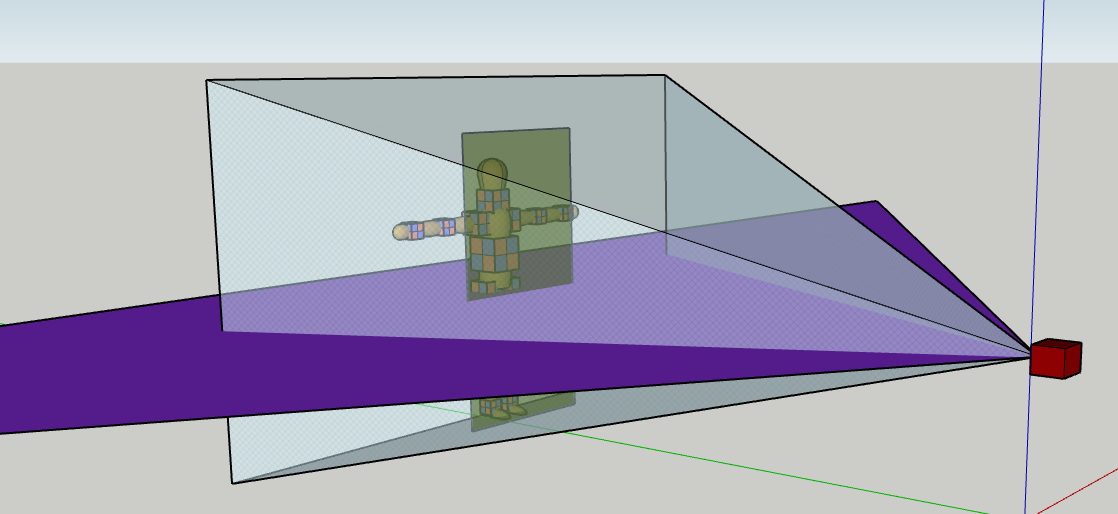
\includegraphics[scale=0.5]{different_dimensions.PNG}
			\captionof{figure}{Visualizing different dimensions measured by the M16 Lidar and Brio Webcam.}
			\label{dimensions}
		\end{figure}


	\subsection{Device Mount}
		Using some spare plywood, I created a mount for the Logitech Brio webcam and Leddar M16 as shown in Figure \ref{mount1}.
		This mount serves to stabilize the webcam and lidar devices in a stationary positions relative to each other so that accurate distance/visual calibrations can be performed.
		If the webcam and lidar devices are not placed in consistent positions, distance information will not be synchronized with object recognition.
		Writing an algorithm to compensate for automatic distance and object recognition calibration is an overly complex task and beyond the scope of this project.

		\begin{figure}[H]
			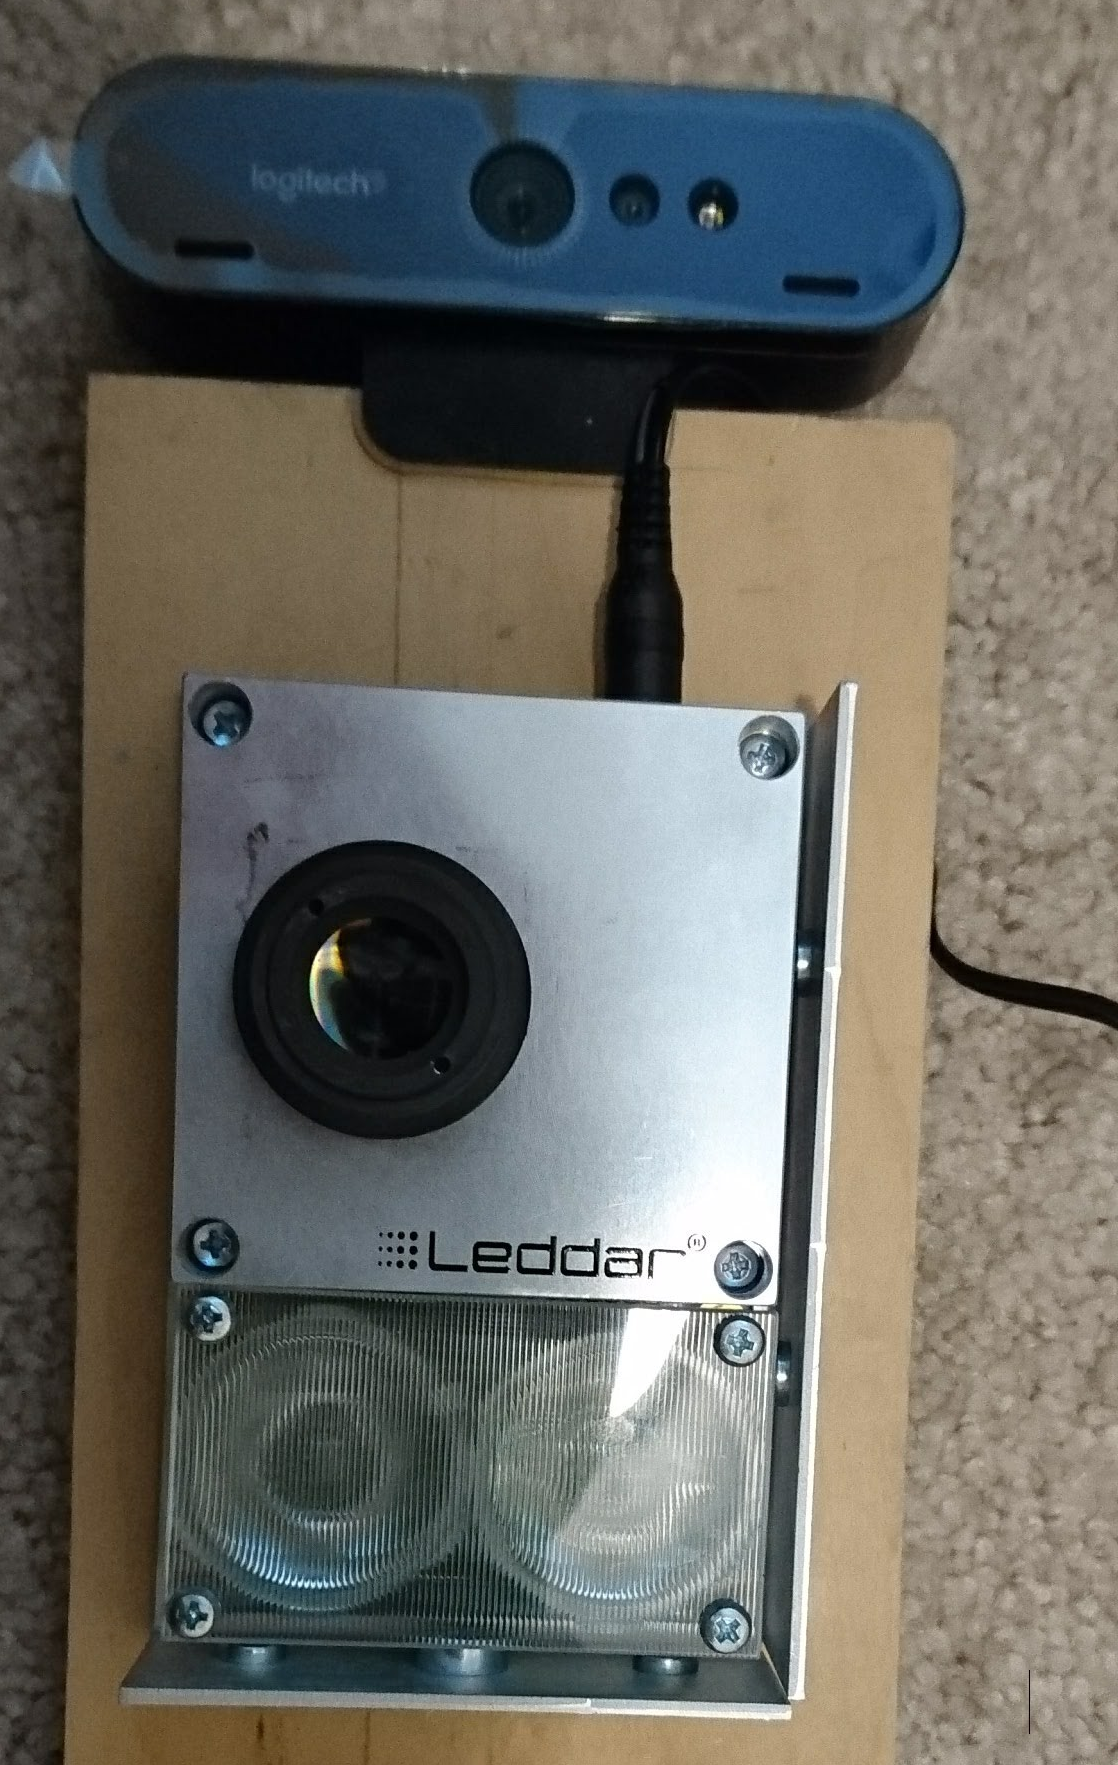
\includegraphics[scale=0.2]{mount1.PNG}
			\captionof{figure}{Part of the mount for .}
			\label{mount1}
		\end{figure}


		Progress with the Leddar M16 is slow and I do not foresee it to be working and integrated in time for expo.
		Fortunately, I was able to read distance information with the RPlidar A1.
		I adjusted the mount to accommodate the RPlidar A1 by drilling a few shallow holes in the base of the mount.
		This allows the RPlidar A1's four plastic standoffs to fit into the base of the mount as shown in Figure \ref{mount2}.

		\begin{figure}[H]
			\includegraphics[scale=0.1]{mount2.PNG}
			\captionof{figure}{Visualizing different dimensions measured by the M16 Lidar and Brio Webcam.}
			\label{mount2}
		\end{figure}

		The device mounting system is complete. 
		Our project's components can be fixed in stable positions to ensure consistent readings in different environments.
		This mounting system is important to our final design because it ensures operational consistency and simplifies the overall problem. 


		\subsection{Computer Vision}
			Over the past term, my contribution towards our proposed design was creating a reliable image-recognition model.
			First, I started with OpenCV's pre-trained facial/pedestrian support-vector-machine (SVM) classifier.
			This SVM is a combination of several other SVMs that detect the upper body, eyes, mouths, and noses.
			The combined SVM is intended to detect faces with high accuracy.
			However, when applied to our design, I could not consistently replicate good results.
			This was due to several factors, namely the SVM used was meant to perform classification on still images where the camera's perspective is far from the subject.
			

			Our design specifications envision a system that quickly tracks multiple subjects in a crowded expo scenario.
			In an expo scenario, human subjects will be moving close or away from the camera, unpredictably shifting their positions, and moving in or out of the field-of-view.
			As seen in \ref{svm}, the OpenCV SVM model does not perform to our specification.
			If the human subject were to turn their head or move too quickly, the SVM will have difficulty tracking their body.
			Additionally, the SVM performs intensive calculations on the computer's CPU, severely limiting the video output's frame-rate and resolution.
			
			\begin{figure}[H]
			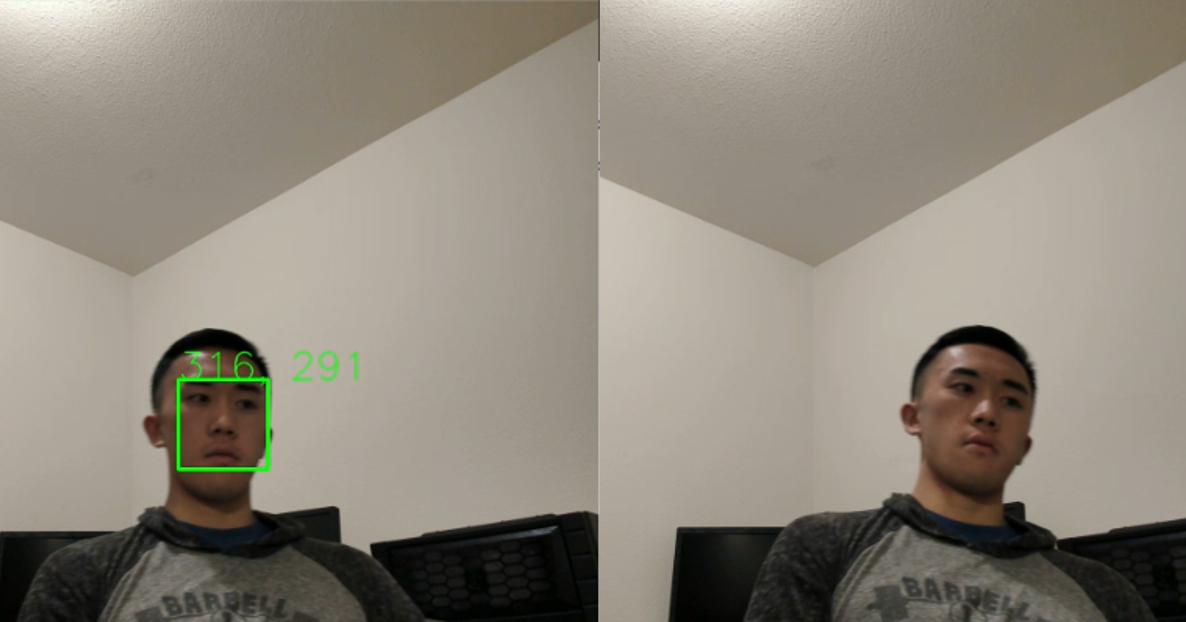
\includegraphics[scale=0.60]{svm.PNG}
			\captionof{figure}{SVM face classification (Left) fails when subject slightly turns their head (Right)}
			\label{svm}
			\end{figure}


			Recognizing the SVM's weaknesses, Tensorflow's open source object detection classifier presented a better computer-vision alternative. \cite{tensorflow}
			The Tensorflow object recognition library is better suited for this project because its library has already been trained to recognize a large dataset of objects. \cite{convolutional_object_detectors}
			These pre-trained datasets in Tensorflow's library are sourced from other machine learning datasets including the COCO dataset, Kitti dataset, and the Open Images dataset. \cite{coco} \cite{open_images} \cite{kitti}


			\begin{figure}[H]
			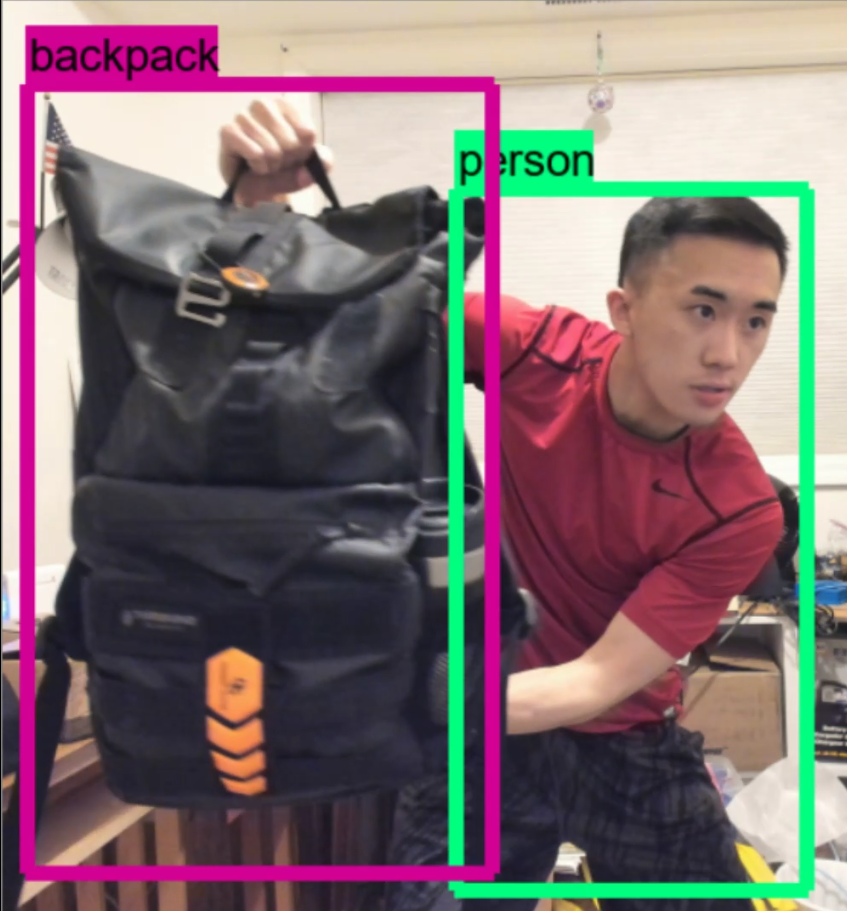
\includegraphics[scale=0.45]{tensorflow.PNG}
			\captionof{figure}{Our pre-trained Tensorflow model can reliably detect multiple subjects}
			\label{tf-detect}
			\end{figure}


			Using this pre-trained Tensorflow model, our project is now able to accurately outline and label over 90 subjects as they come into view of the webcam.
			In addition to compiling this Tensorflow model, I have also prepared our code for when we eventually create the depth-sensing component of our project.
			The current state of the code will enable us to selectively edit the output video frames to draw bounding boxes on subjects as they move in and out of the camera's field of view.


			Tensorflow also enables us to take advantage of NVIDIA CUDA, a driver that moves intensive calculations to the GPU.
			While this increases our list of material requisitions for our physical expo demo, moving calculations to the GPU greatly improves the output video quality, frame rate, resolution, and classification speed. \cite{nvidia}
			The computer vision aspect of our project is now complete.
			Combined with a stable mount, we now have a versatile system that can recognize over 80 distinct models such as humans, bags, or animals in near real-time.
			

	\clearpage

\end{singlespace}
\end{document}
